\documentclass{article}
\usepackage[utf8]{inputenc}
\author{Kevin Liu, Kenneth Yu, and Tim Qin}
\date{May 18, 2018}
\title{Eutrophication}
\usepackage{amsmath, chemfig, subcaption, caption, graphicx, lmodern}
\usepackage[version=4]{mhchem}
\usepackage{biblatex}
\addbibresource{references.bib}
\graphicspath{ {./images/} }
\begin{document}
\maketitle
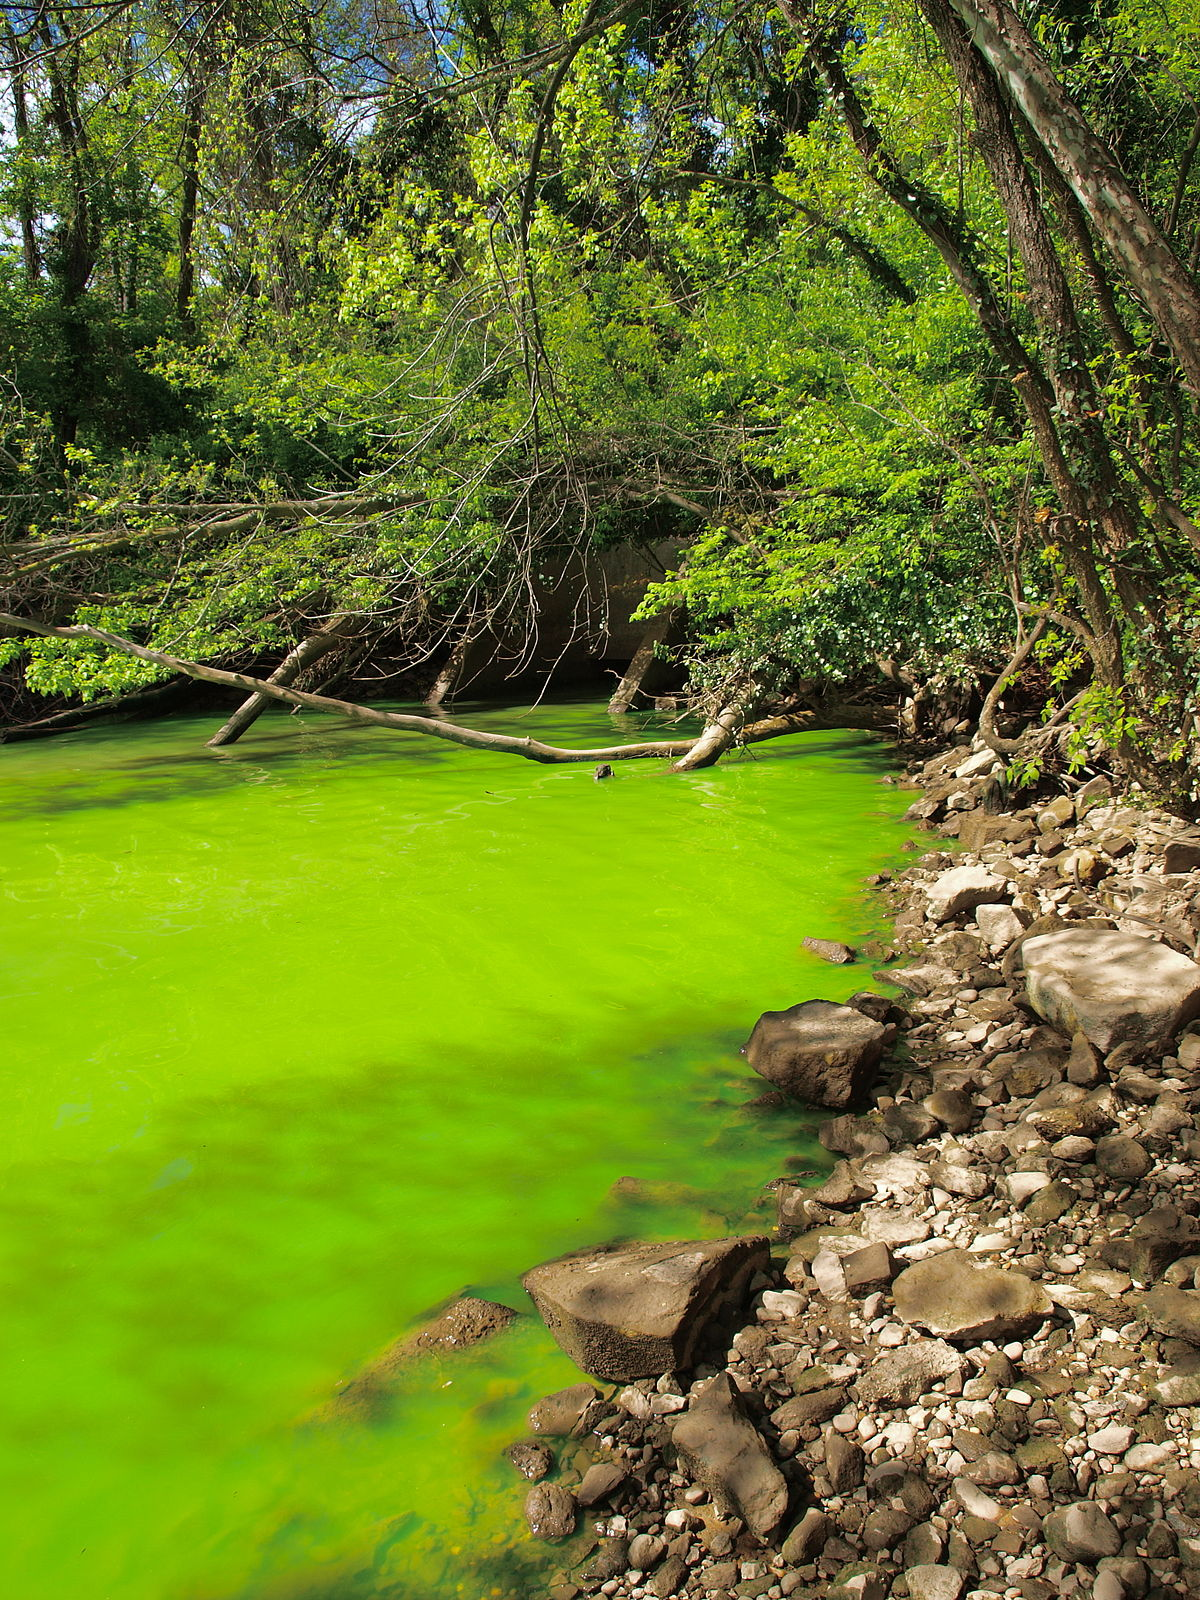
\includegraphics[scale=.25]{TitlePic}
\pagenumbering{gobble}
\clearpage
\tableofcontents
\listoffigures
\clearpage
\pagenumbering{arabic}
\section{Introduction}
Eutrophication (from the Greek $\epsilon\Tilde{\upsilon}  + \tau\rho o \phi\Acute{\eta}$, "well nourished") is a phenomenon that occurs when a body of water becomes overly rich with minerals and nutrients that encourage excessive growth of plants or algae.
This process may lead to oxygen depletion of the water if the amount of oxygen consumed by decomposers overtakes the amount created by producers. 
Eutrophication is usually caused by the discharge of nitrate or phosphate-containing detergents, fertilizers or sewage into an aquatic system\cite{wikipedia}.
\section{Cause}
Eutrophication is caused by the release of either nitrates ($\ce{NO3^2-}$) or phosphates($\ce{PO4^3-}$) into aquatic environments by the results of human activities.
These two chemicals are usually the limiting factors for algae and plant growth, and the addition of these chemicals causes the producers to enter their exponential growth phase, in which growth is governed by
\begin{align}
    \frac{dN}{dt} = r_{max}N
\end{align}
These producers eventually die off, usually very close to each other, and increase oxygen consumption through decomposition.
\begin{figure}[h]
    \begin{subfigure}{.5\textwidth}
        \centering
        \chemfig{P(=[:90,.75]O)(<:[:350]O^{-})(<[:280,.75]O^{-})(-[:200,.75]O^{-})}
        \caption{Phosphate}
    \end{subfigure}%
    \begin{subfigure}{.5\textwidth}
        \centering
        \chemfig{N(=[:90,.75]O)(-[:210,]O^{-})(-[:330,]O^{-})}
        \caption{Nitrate}
    \end{subfigure}
    \caption{Chemicals that cause eutrophication}
\end{figure}
    \subsection{Cellular Respiration}
    It is through cellular respiration that Oxygen depletion occurs during eutrophication. 
    After the producers created by eutrophication die off, the population of the detritivore population increases dramatically, and with it, an increased occurrence of cellular respiration.
    \begin{align}
        \ce{C6H12O6 + 6O2 -> 6H2O + 6CO2 + ATP}
    \end{align}
    Since the detritivore population increases while the producer population decreases, there is more $\ce{O2}$ consumed then there is being produced. Once the oxygen level is low enough, the detritivores start to die off, leaving a eutrophic environment.
\section{Consequences}
The effects of eutrophication, including increases in $\ce{CO2}$ and increased amounts of dissolved solutes in the water, have many consequences, of which some are a more acidic environment, less oxygen-carrying capacity, and increased ammonia level.
    \subsection{Decreasing pH}
    The increases in $\ce{CO2}$ levels means that the amount of $\ce{H2CO3}$ formed also increases. 
    \begin{align}
        \ce{H2O + CO2 -> H2CO3}
    \end{align}
    Since $\ce{H2CO3}$ is a weak acid, a portion of the Carbonic acid molecules will disassociate into $\ce{H+ + CO3-}$
    \begin{align}
        \ce{H2CO3 <=> H+(aq) + HCO3-(aq)}
    \end{align}
    \subsection{Reduction of the population of organisms}
    The bloom and subsequent die-off of aquatic plants, algae, and cyanobacteria and the ensuing depletion of oxygen are similar to what occurs in marine dead zones. 
    Such conditions threaten the survival of organisms. One example is of Lake Erie, in which eutrophication coupled with overfishing wiped out the populations of pike, whitefish, and trout by the 1960's\cite{bio}.
        \begin{figure}[h]
            \centering
            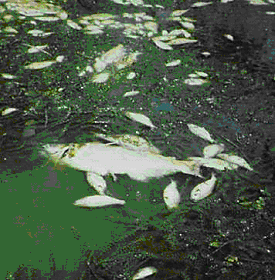
\includegraphics{deadfish}
            \caption{One consequence of eutrophication}
            \label{fig:deadfish}
        \end{figure}
\newpage
\printbibliography[heading=bibintoc]
\end{document}